\pagebreak
\section{Magnetometer Calibration} \label{app:magnetoCalibration}
\textbf{Name: Group 510}\\
\textbf{Date: 26/11 - 2015}

\subsection{Purpose}
The purpose of this test is to ensure the fact that the magnetometer is calibrated so that it can tell a correct position relative to the Earth's magnetic field when placed on the vehicle.

\subsection{Theory}
The HMC5883L chip \cite{HMC5883L} is a magnetometer which uses the Earth's magnetic field as a reference. When using it for the first time it is necessary to calibrate it so that disturbances in the close field of the sensor are accounted for in later measurements.\\
%
In this project the disturbances can be caused by all the metallic pieces on the vehicle, from the metal plate to the motor and to the wires. Thus, the calibration has to be performed with the all these components and the sensor placed on the vehicle at a fixed place and orientation. It is chosen to place it, so that its X axis points towards the front of the vehicle and the Z axis is pointed upwards. The chosen configuration shall not be changed after calibration.

As stated in \secref{sec:magnetoSensor}, the magnetometer that is used gives out three space coordinates of the Earth's magnitude field relative to its own coordinate system. One good test to see if the sensor is operational in its environment is to turn it all around itself while retrieving the data it gives. When properly calibrated and isolated from any new disturbance, the 3D scatter plot of all the measured points should give a sphere that has its center in the origin (coordinates (0,0,0)) of the plot. This means that the measured coordinates vary smoothly accordingly with the rotation of the sensor in space. Otherwise, the sphere could be distorted into an ellipsoid and displaced from the center and the sensor would have to be recalibrated correctly in a magnetic-still environment, see example with the magnetometer alone on \figref{fig:calibrationTestSpheres}.\\
A simpler test is used here to check for the good calibration with the vehicle. It consists in making four quarters of turn in the XY-plane (horizontally), around a static point. If each quarter corresponds to a measurement of \si{90^{\circ}} in the sensor's data and the resulting four quarters draw a circle, then the calibration is fine to use.
\begin{figure}[H]
    \centering
  %Trim margins @:   left        bottom       right       top
  \adjustbox{ trim = {.1\width} {0.03\height} {0\width} {0.1\height}, clip }
  {
    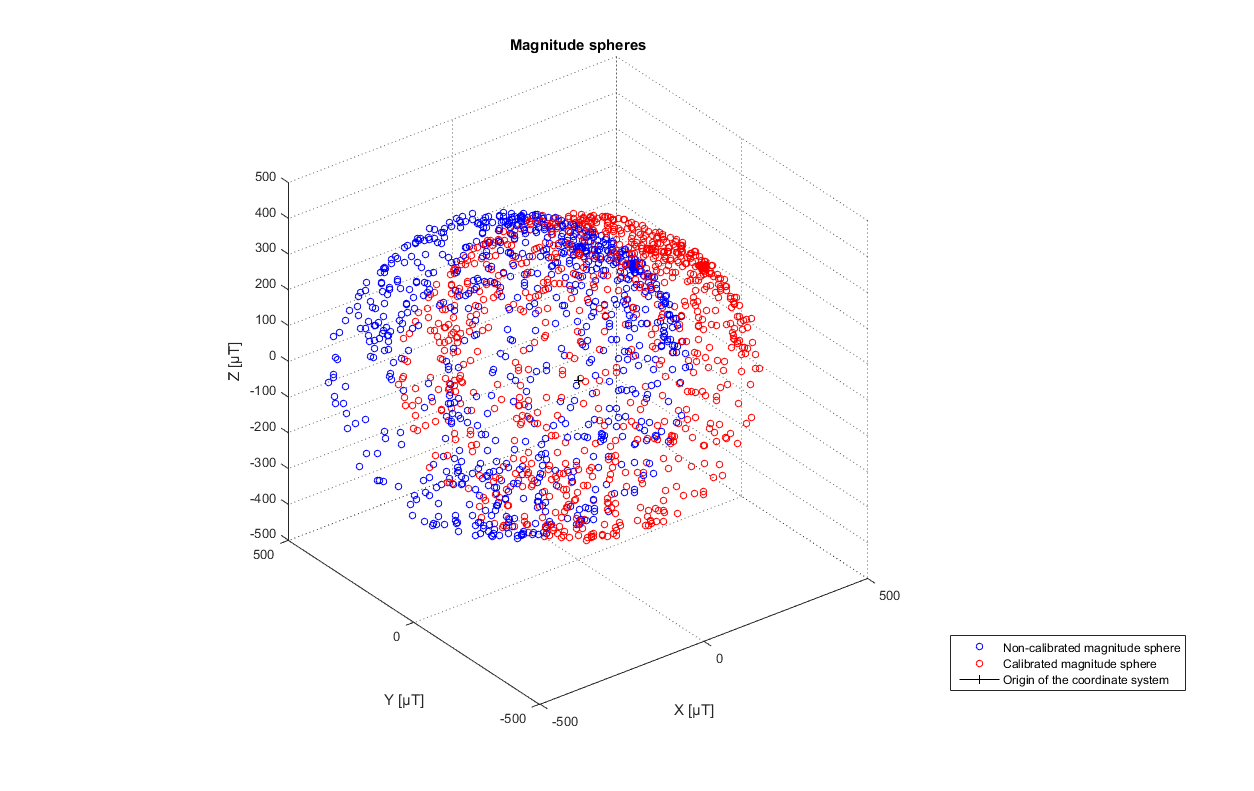
\includegraphics[width=1.2\textwidth]{figures/spheresMagnitude.png}
  }
  \caption{Magnetic sphere of calibrated and non-calibrated sensor alone}
  \label{fig:calibrationTestSpheres}
\end{figure}
\todo{Change units to Gauss}
%
The calibration itself performed in this test does not change the intrinsic sensor configuration but rather applies a transformation to the coordinates sent to the Arduino board. This transformation, seen in \eqref{eq:calibrationTransformation} is actually computed in the runtime by the microcontroller, each time a set of coordinate is received :
\begin{flalign}
  \eq{X_{cal}}{M \cdot X_{measured} + B}\unit{G}
  \label{eq:calibrationTransformation}
\end{flalign}
\hspace{6mm} Where:\\
\begin{tabular}{p{1cm}lll}
& \si{X_{cal}}      & is a $3\times 1$ vector of calibrated coordinates     &\unitWh{G}\\
& \si{M}            & is a $3\times 3$ transformation matrix                &\unitWh{\cdot}\\
& \si{X_{measured}} & is a $3\times 1$ vector of non-calibrated coordinates &\unitWh{G}\\
& \si{B}            & is a $3\times 1$ bias vector                          &\unitWh{G}
\end{tabular}

The transformation matrix, M, allows for the transformation of an ellipsoid into a proper sphere, while the bias vector shifts the resulting sphere to the center of the sensor's coordinate system. The expanded matrix form is the following :
\begin{flalign}
  \begin{pmatrix}
    \si{x_{cal}} \\
    \si{y_{cal}} \\
    \si{z_{cal}} 
  \end{pmatrix}
  &=
  \begin{pmatrix} 
    \si{m_{1,1}} & \si{m_{1,2}} & \si{m_{1,3}} \\
    \si{m_{2,1}} & \si{m_{2,2}} & \si{m_{2,3}} \\
    \si{m_{3,1}} & \si{m_{3,2}} & \si{m_{3,3}} 
  \end{pmatrix}
  \cdot
  \begin{pmatrix} 
    \si{x_{measured}} \\
    \si{y_{measured}} \\ 
    \si{z_{measured}} 
  \end{pmatrix} 
  + 
  \begin{pmatrix} 
    \si{b_x} \\ 
    \si{b_y} \\ 
    \si{b_z} 
  \end{pmatrix}\unit{G}
  \label{eq:calibrationTransformationExpanded}
\end{flalign}
Each set of measured space coordinates, \si{X_{measured}}, is put into \eqref{eq:calibrationTransformationExpanded}. The coefficients of the transformation matrix, M, and of the bias vector, B, are found from a dedicated software, MagMaster \cite{MagMaster}.\\
This software, runs on Microsoft Windows computers with the HMC5883L sensor connected through an Arduino. It requires to put the sensor in different pre-defined positions, so that it points towards all the axis successively, and finally computes the needed values. The latter finally have to be put into the software that needs use the magnetometer readings and applies the desired calculations.

%% Test setup description %%
\subsection{Setup}
\begin{figure}[H]
  \centering
  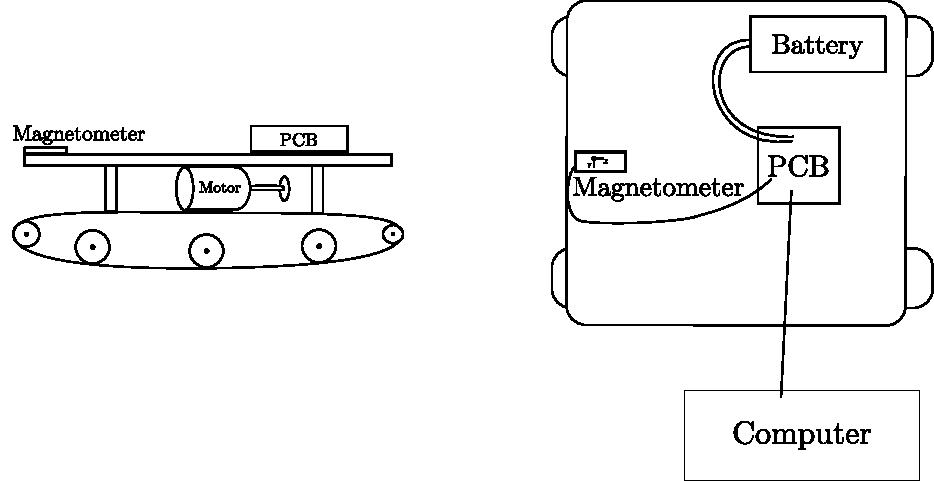
\includegraphics[scale=0.8]{figures/magnetoCalibSetup.pdf}
  \caption{Setup diagram}
  \label{fig:calibrationSetupDiagram}
\end{figure}
\todo{Change units to Gauss}

\subsection{List of Equipment}

\begin{table}[H]
\begin{tabular}{|p{10cm}|p{4cm}|}
\hline%------------------------------------------------------------------------------------
  \textbf{Instrument}                     &  \textbf{Type}       \\
\hline%------------------------------------------------------------------------------------
  Computer                                &  HP 8460P            \\
\hline %-----------------------------------------------------------------------------------
\end{tabular}
\end{table}

%% Procedure %%
\subsection{Procedure}

\begin{enumerate}
  \item Set up the vehicle and the hardware so that the magnetometer is far from other non-constant magnetic objects (motor, PCB, wires) and with the X arrow pointing towards the front of the vehicle and the Z pointing upwards.
  \item Attach everything, including the wires and serial USB cable, as it is, so that it cannot move. The configuration should stay the same as long as the magnetometer is used, otherwise, it has to be re-calibrated.
  \item Put the vehicle in the environment in which the magnetometer has to operate.
  \item Plug the sensor to the Arduino board and the Arduino to the computer via the USB serial cable.
  \item Run the MagMaster software.
  \item Select the right USB serial port.
  \item Start the measurements by putting the vehicle in the position indicated by the software tutorial \cite{MagMaster}. Click on the associated measurement button.
  \item While performing the test, make sure that no magnetic part is moving (especially the USB cable).
  \item When all positions are measured thourgh the software, it is possible to unplug the serial connection with the Arduino.
  \item Click on `Calculate Transformation Matrix and Bias'.
  \item Write down the calculated coefficients for later reference and put them in the Arduino sensor code.
  \item Test the sensor by using the four-quarters of turn method.
\end{enumerate}

%% Results %%
\subsection{Results} \label{magnetoCalibrationResults}
After having done the measurements and computed the transformation matrix and bias vector with the software, with the magnetometer on the vehicle, the coefficients used further on in the code are :
 \begin{flalign}
  M &= 
  \begin{pmatrix} 
    \si{1,206} & \si{-0,002} & \si{0,039} \\
    \si{0,013} & \si{1,193} & \si{-0,004} \\
    \si{-0,004} & \si{-0,025} & \si{1,414} 
  \end{pmatrix}\unit{G}
\end{flalign}
\begin{flalign}
  B =
  \begin{pmatrix} 
    \si{-52.455,}\\
    \si{-164.666}\\
    \si{-143.707}
  \end{pmatrix}\unit{G}
  \label{eq:calibrationTransformationExpanded}
\end{flalign}

The four-quarters of turn test made with these settings is illustrated in \figref{fig:calibrationTestQuarterResults}.
\begin{figure}[H]
    \centering
  %Trim margins @:   left        bottom       right       top
  \adjustbox{ trim = {.1\width} {0.15\height} {0\width} {0.1\height}, clip }
  {
    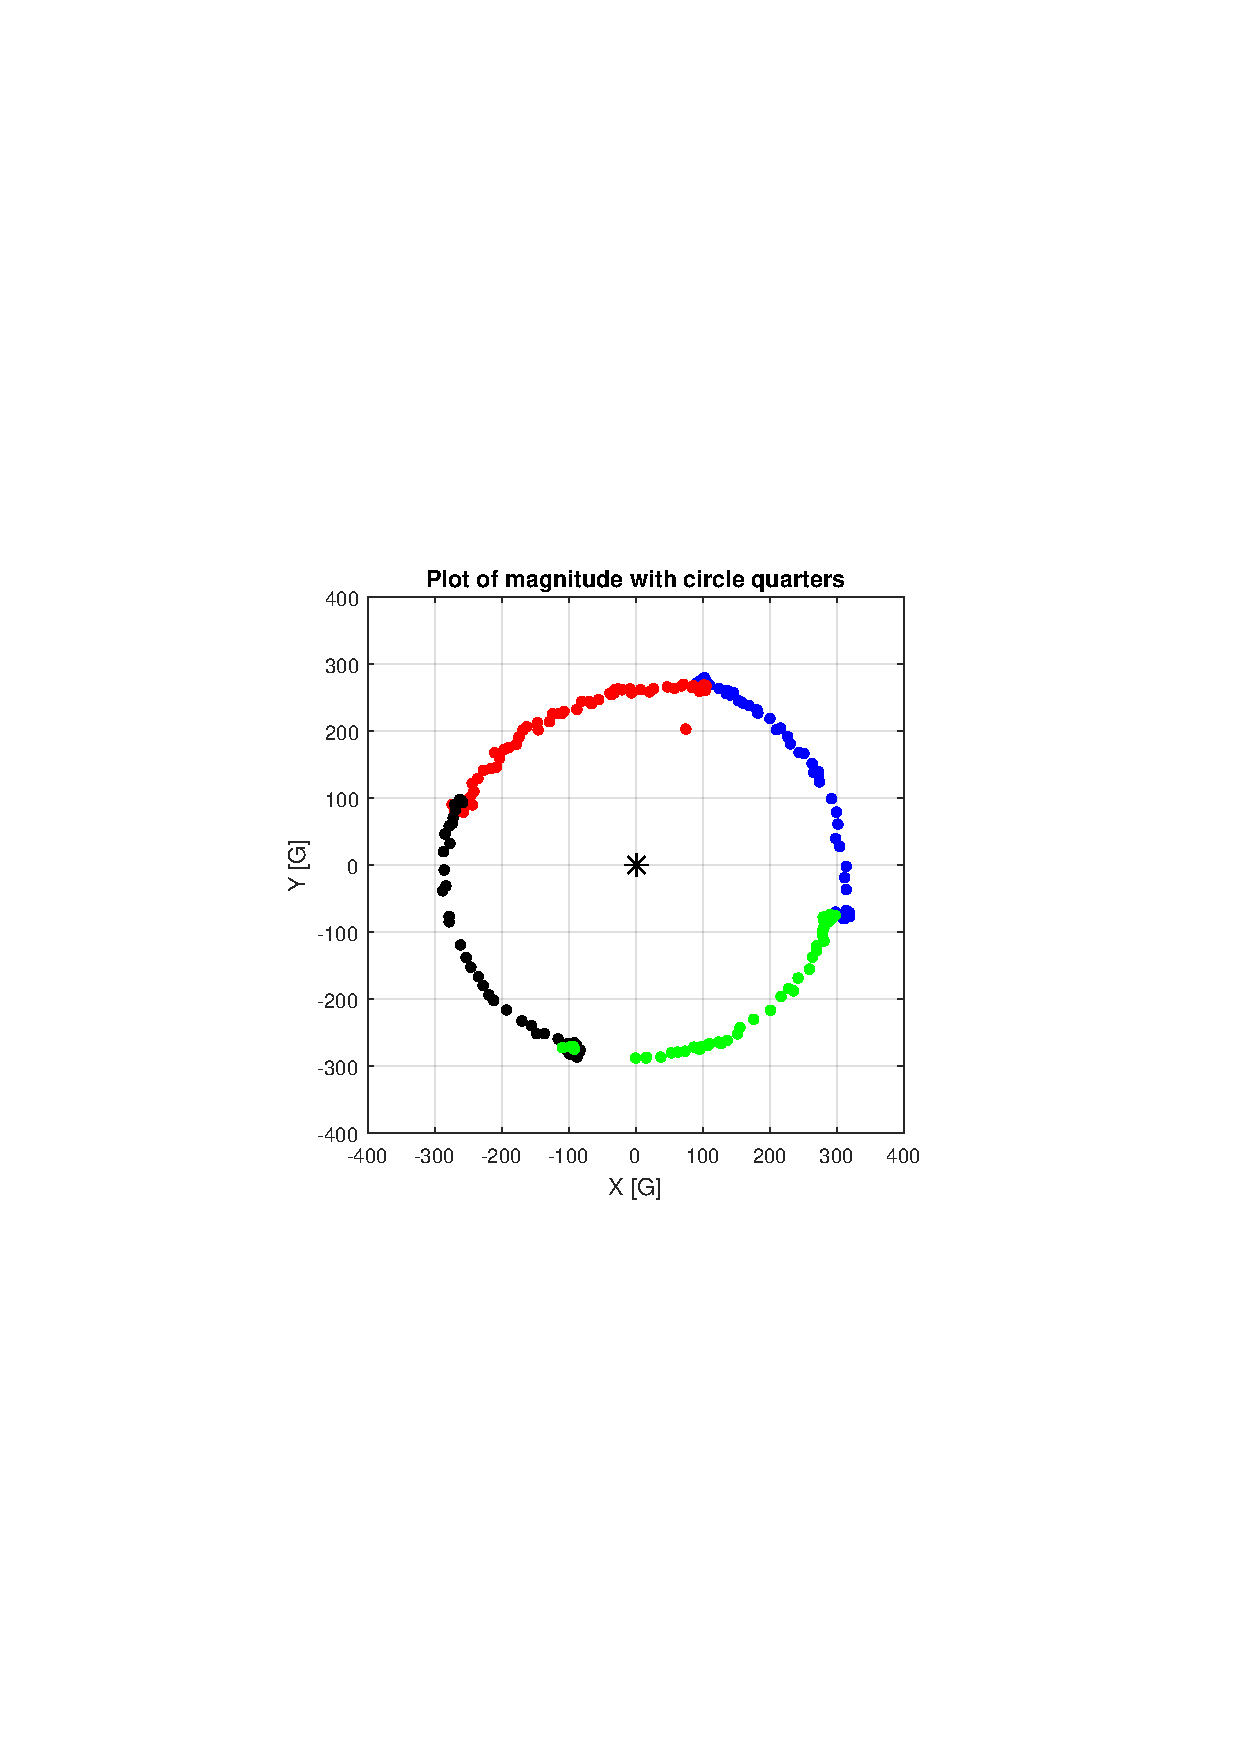
\includegraphics[width=0.9\textwidth]{figures/fullturn2.pdf}
  }
  \caption{Test of the calibrated sensor onboard the vehicle with four quarters of turn}
  \label{fig:calibrationTestQuarterResults}
\end{figure}
\todo{Correct axis and title + add a cross}

The cross on \figref{fig:calibrationTestQuarterResults} has right angles and passes through the center of the circle which is in (0,0). This shows that each quarter of turn in reality is measured by \si{90^{\circ}} by the sensor and that the latter is correctly calibrated for use on the vehicle.